\documentclass[10pt, conference, letterpaper]{IEEEtran}

\usepackage{algorithm}
\usepackage{algorithmicx}
\usepackage{algpseudocode}
\usepackage{amsfonts}
\usepackage{amsmath}
\usepackage{amssymb}
\usepackage[ansinew]{inputenc} 
\usepackage{xcolor}
\usepackage{mathtools}
\usepackage{graphicx}
\usepackage{caption}
\usepackage{subcaption}
\usepackage{import}
\usepackage{multirow}
\usepackage{cite}
\usepackage[export]{adjustbox}
\usepackage{breqn}
\usepackage{mathrsfs}
\usepackage{acronym}
%\usepackage[keeplastbox]{flushend}
\usepackage{setspace}
\usepackage{bm}
\usepackage{stackengine}
\usepackage{dirtytalk}
\usepackage{tipa}

\usepackage{listings}

\lstset{%
 backgroundcolor=\color[gray]{.85},
 basicstyle=\small\ttfamily,
 breaklines = true,
 keywordstyle=\color{red!75},
 columns=fullflexible,
}%

\lstdefinelanguage{BibTeX}
  {keywords={%
      @article,@book,@collectedbook,@conference,@electronic,@ieeetranbstctl,%
      @inbook,@incollectedbook,@incollection,@injournal,@inproceedings,%
      @manual,@mastersthesis,@misc,@patent,@periodical,@phdthesis,@preamble,%
      @proceedings,@standard,@string,@techreport,@unpublished%
      },
   comment=[l][\itshape]{@comment},
   sensitive=false,
  }

\usepackage{listings}

% listings settings from classicthesis package by
% Andr\'{e} Miede
\lstset{language=[LaTeX]Tex,%C++,
    keywordstyle=\color{RoyalBlue},%\bfseries,
    basicstyle=\small\ttfamily,
    %identifierstyle=\color{NavyBlue},
    commentstyle=\color{Green}\ttfamily,
    stringstyle=\rmfamily,
    numbers=none,%left,%
    numberstyle=\scriptsize,%\tiny
    stepnumber=5,
    numbersep=8pt,
    showstringspaces=false,
    breaklines=true,
    frameround=ftff,
    frame=single
    %frame=L
}

\renewcommand{\thetable}{\arabic{table}}
\renewcommand{\thesubtable}{\alph{subtable}}

\DeclareMathOperator*{\argmin}{arg\,min}
\DeclareMathOperator*{\argmax}{arg\,max}

\def\delequal{\mathrel{\ensurestackMath{\stackon[1pt]{=}{\scriptscriptstyle\Delta}}}}

\graphicspath{{./figures/}}
\setlength{\belowcaptionskip}{0mm}
\setlength{\textfloatsep}{8pt}

\newcommand{\eq}[1]{Eq.~\eqref{#1}}
\newcommand{\fig}[1]{Fig.~\ref{#1}}
\newcommand{\tab}[1]{Tab.~\ref{#1}}
\newcommand{\secref}[1]{Section~\ref{#1}}

\newcommand\MR[1]{\textcolor{blue}{#1}}
\newcommand\red[1]{\textcolor{red}{#1}}
\newcommand{\mytexttilde}{{\raise.17ex\hbox{$\scriptstyle\mathtt{\sim}$}}}

%\renewcommand{\baselinestretch}{0.98}
% \renewcommand{\bottomfraction}{0.8}
% \setlength{\abovecaptionskip}{0pt}
\setlength{\columnsep}{0.2in}

% \IEEEoverridecommandlockouts\IEEEpubid{\makebox[\columnwidth]{PUT COPYRIGHT NOTICE HERE \hfill} \hspace{\columnsep}\makebox[\columnwidth]{ }} 

\title{Attention Based Models for Keyword Spotting\\}

\author{Riccardo Mazzieri
%	$^\dag$
%\thanks{$^\dag$Department of Information Engineering, University of Padova, email: \{rossi\}@dei.unipd.it}
} 

\IEEEoverridecommandlockouts

\newcounter{remark}[section]
\newenvironment{remark}[1][]{\refstepcounter{remark}\par\medskip
   \textbf{Remark~\thesection.\theremark. #1} \rmfamily}{\medskip}

\begin{document}

\maketitle

\begin{abstract}
	%TODO
In this work we explore a variety of Deep neural newtork architectures, with particular focus on the attention mechanism, for the Keyword Spotting task (KWS). In recent years, attention based models have proven to be successful in a wide variety of domains, including image recognition, neural machine translation and speech recognition. We analyize recent attention based architectures: we first focus on the model proposed by de Andreade et al, and explore the role of the size of filters in the convolutional part of the model.
\end{abstract}

\IEEEkeywords
Keyword Spotting, Convolutional Neural Networks, Recurrent Neural Networks, Attention Mechanism, Transformers. 
%\MR{A list of keywords defining the tools and the scenario. I would not go beyond {\it six} keywords.}
\endIEEEkeywords


\input{Intro}

% !TEX root = template.tex

\section{Related Work}
\label{sec:related_work}

\noindent \textbf{Some hints:} 
\begin{itemize}
\item \textbf{Goal:} The goal of this section is to describe what has been done so far in {\it the} literature. You should focus on and briefly describe the work done in the best papers that you have read. 
\item \textbf{Length:} One full column is fine but often this takes one column and a half. It is very easy to use a full page, although this may just due to your sloppiness... if you carefully go through the one page long version, you often find it possible to compact it in one column and a half. In any event, I would make this section no longer than one page, this leads to an overall {\it two pages} including abstract, introduction and related work. I believe this is a fair amount of space in most cases.
\item \textbf{Approach:} For each you should comment on the paper's contribution, on the good and important findings of such paper and also, \textbf{1)} on why these findings are not enough and \textbf{2)} how these findings are improved upon/extended by the work that you present here. At the end of the section, you may recap the main paper contributions (maybe one or two, the most important ones) and how these extend/improve upon previous work.
\end{itemize}
\begin{itemize}
\item \textbf{References:} please follow this {\it religiously}. It will help you a lot. Use the Latex \texttt{Bibtex} tool to manage the bibliography. A \texttt{Bibtex} example file, named \texttt{biblio.bib} is provided with this template.\\

\item \textbf{Citing conference/workshop papers:} I recommend to always include the following information into the corresponding \texttt{bibitem} entry: 
\begin{enumerate}
\item author names, 
\item paper title, 
\item conference / workshop name, 
\item conference / workshop address, 
\item month, 
\item year.
\end{enumerate}
Examples of this are: \cite{Zargham-2011}\cite{Sadler-2006}.\\

\item \textbf{Citing journal papers:} I recommend to always include the following information into the corresponding \texttt{bibitem} entry: 
\begin{enumerate}
 \item author names, 
 \item paper title, 
 \item full journal name, 
 \item volume (if available), 
 \item number (if available), 
 \item month, 
 \item pages (if available), 
 \item year. 
 \end{enumerate}
 Examples of this are: \cite{Shannon-1948}\cite{Boyd-2011}\cite{Zordan-2014}.\\

\item \textbf{Citing books:} I recommend to always include the following information into the corresponding \texttt{bibitem} entry: 
\begin{enumerate}
\item author names, 
\item book title, 
\item editor, 
\item edition, 
\item year.
\end{enumerate}
\end{itemize}
%

\begin{remark}
Note that some of the above fields may not be shown when you compile the Latex file, but this depends on the bibliography settings (dictated by the specific Latex style that you load at the beginning of the document). You may decide to include additional pieces of information in a given bibliographic entry, but please, \textbf{be consistent} across all the entries, i.e., use the same fields for the same publication type. Note that some of the fields may not be available (e.g., the paper {\it volume}, {\it number} or the {\it pages}).
\end{remark}

% !TEX root = project_report.tex
\section{Experimental Setup}

\subsection{Signals and Features}
\label{sec:sig&features}

%Com'è , il dataset, che tipo di features uso, spiegare come sono estratte, spiegare augmentation strategies, spiegare come genero gli split del dataset per ogni task.

Each model was trained on the Google Speech Commands dataset V2 \cite{speechdataset2018warden}, which consists on a total of $105829$ user utterances of a total of $35$ keywords. Each utterance is stored as a one second long\footnote{Some clips are a bit shorter than one second: in those cases, the clips are zero padded towards the end.} \verb|WAVE| file, sampled at a 16KHz rate. From each signal, $40$ MFCCs are computed, using a window size of $25$\textit{ms} ($400$ samples) and a hop size of $10$\textit{ms} ($160$ samples). With this approach, the input for the network consists in 3D tensors with one outer channel, where width represents the time domain and height represents the frequency domain. Following Google's suggestions from \cite{speechdataset2018warden}, the dataset is split in 80\% for training set, 10\% for validation set and 10\% for test set, in such a way that the same speakers are never present in two different splits. 
Following the approach from past literature, the models are trained for two different tasks, which are the following:
\begin{itemize}
	\item \textbf{12kws} task: the model must discriminate among 12 different keywords: \say{yes}, \say{no}, \say{up}, \say{down}, \say{left}, \say{right}, \say{on}, \say{off}, \say{stop}, \say{go}, unknown or silence. The unknown keywords are randomly chosen from the set of remaining keywords and the silence samples consist in one second long crops, randomly extracted from the noise files provided by the dataset\footnote{Those consist in 6 files containing noisy background sounds, both artificially generated and recorded from real environments.}. Since the total amount of words belonging to the \say{unknown} class was much higher than the number of representatives for each of the other keywords, we decided to randomly extract them to create a balanced dataset. In this way, we have 36921 samples for training, 4443 for validation and 4888 for testing.
	\item \textbf{35kws} task: the model must discriminate among all the 35 keywords present in the dataset. No unknown class or silence class is introduced, therefore, for this task, the entire dataset is used. The training set consists in 84843 samples, the validation set in 9981 samples and the test set in 11005 samples. 
\end{itemize}


For each task, the training set is augmented, following existing approaches from the literature. Specifically, the augmentation process follows this order:
\begin{enumerate}
	\item Each signal is randomly shifted left or right (zero padding the remaining portion), by $x$ \textit{ms}, where $x$ is drawn from a uniform distirbution $U(0,100)$;
	\item Samples belonging to the \say{silence} class do not remain the same across epochs, but are randomly generated each time;
	\item With a probability of $0.8$, each signal is mixed with a randomly generated background noise, which is multiplied by a factor drawn from $U(0,0.2)$; 
	\item After the conversion in MFCC, the features are augmented using SpecAugment \cite{park2019specaugment}, a simple data augmentation method which consists in adding randomly sized frequency and time masks to the feature matrix: this is done in order to render the model more robust to partial loss of frequency information or of small sections of speech. We set the maximum size for the time and frequency mask equal to $20$ and $10$ respectively.
\end{enumerate}

The image resulting from the last step constitutes the actual input for the model. Specifically, each image is a $98 \times 40$ matrix, where the $i$-th row represents the MFCCs of the $i$-th time frame. 

%We remark that validation and test sets are not touched by the augmentation process.

All the project was carried out using an NVIDIA GeForce GTX 1060 6GB GPU and an Intel i5-64000 CPU, on a Linux machine. All models were built and trained using TensorFlow~\cite{Abadi2016TensorFlowAS}. All source code is available on Github\footnote{\url{https://github.com/rmazzier/HDA-Project-Key-Word-Spotting}}.

\subsection{Input Pipeline}
\label{sec:processing_architecture}
%\textbf{Why having this section:} With this section, we start the technical description with a {\it high level} introduction of your work (e.g., processing pipeline). Here, you do not have to necessarily go into the technical details of every block/algorithm of your design, this will be done later as the paper develops. What I would like to see here is a high level description of the approach, i.e., which processing blocks you used, what they do (in words) and how these were combined, etc. This section should introduce the reader to your design, explain the different parts/blocks, how they interact and why. You should not delve into technical details for each block, but you should rather explain the big picture. \MR{Besides a well written explanation, I often use a nice diagram containing the various blocks and detailing their interrelations.}
Since data augmentation is applied, storing the entire dataset in memory would not be possible: this would result in the same data being reused across epochs. For this reason, a core part of this work was to build an efficient input pipeline that could handle data augmentation on the fly, during training. In this section we explain how the data generation pipeline works. The augmentation takes place in two different moments during training: 
\begin{enumerate}
	\item Phase 1: here, for each sample beloging to the \textit{silence} class, random noise clips are extracted; also, each sample is randomly shifted. This is performed by the CPU, while the GPU is performing training. 
	\item Phase 2: this phase is performed inside the model by the GPU, with a series of preprocessing layers. Specifically, several custom preprocessing layers were built:
	%TODO add descriptions for each of them e default hyperparameters!
	\begin{enumerate}
		\item \verb|RandomNoiseAugment|: takes care of randomly adding noise to each waveform;
%		\item \verb|LogMelSpectrogram|: converts each waveform to its respective log-mel spectrogram;
		\item \verb|MFCC|: converts each waveform to its respective MFCC matrix;
		\item \verb|SpecAugment|: performs the data augmentation following the SpecAugment policy.
	\end{enumerate}
\end{enumerate}

Note that, in Phase 1, each operation is performed one sample at a time, while in Phase 2 each operation is performed in parallel on an entire batch of samples: this results in a much more optimized implementation. Given the hardware setup with which the project was carried on, this framework was a necessity: just computing the MFCCs for each sample on CPU caused a performance bottleneck, wasting the computational capabilities of the GPU. In Figure \ref{fig:inputpipeline} we report a detailed diagram, showing all the steps in the input pipeline for the generation of the training set. For the validation and test sets, the augmentation is not applied. Furthermore, to ensure complete separation between training and validation/test sets, the noise samples were generated from different portions of the noise files, based on whether or not they were used for training.

\begin{figure}
	\centering
	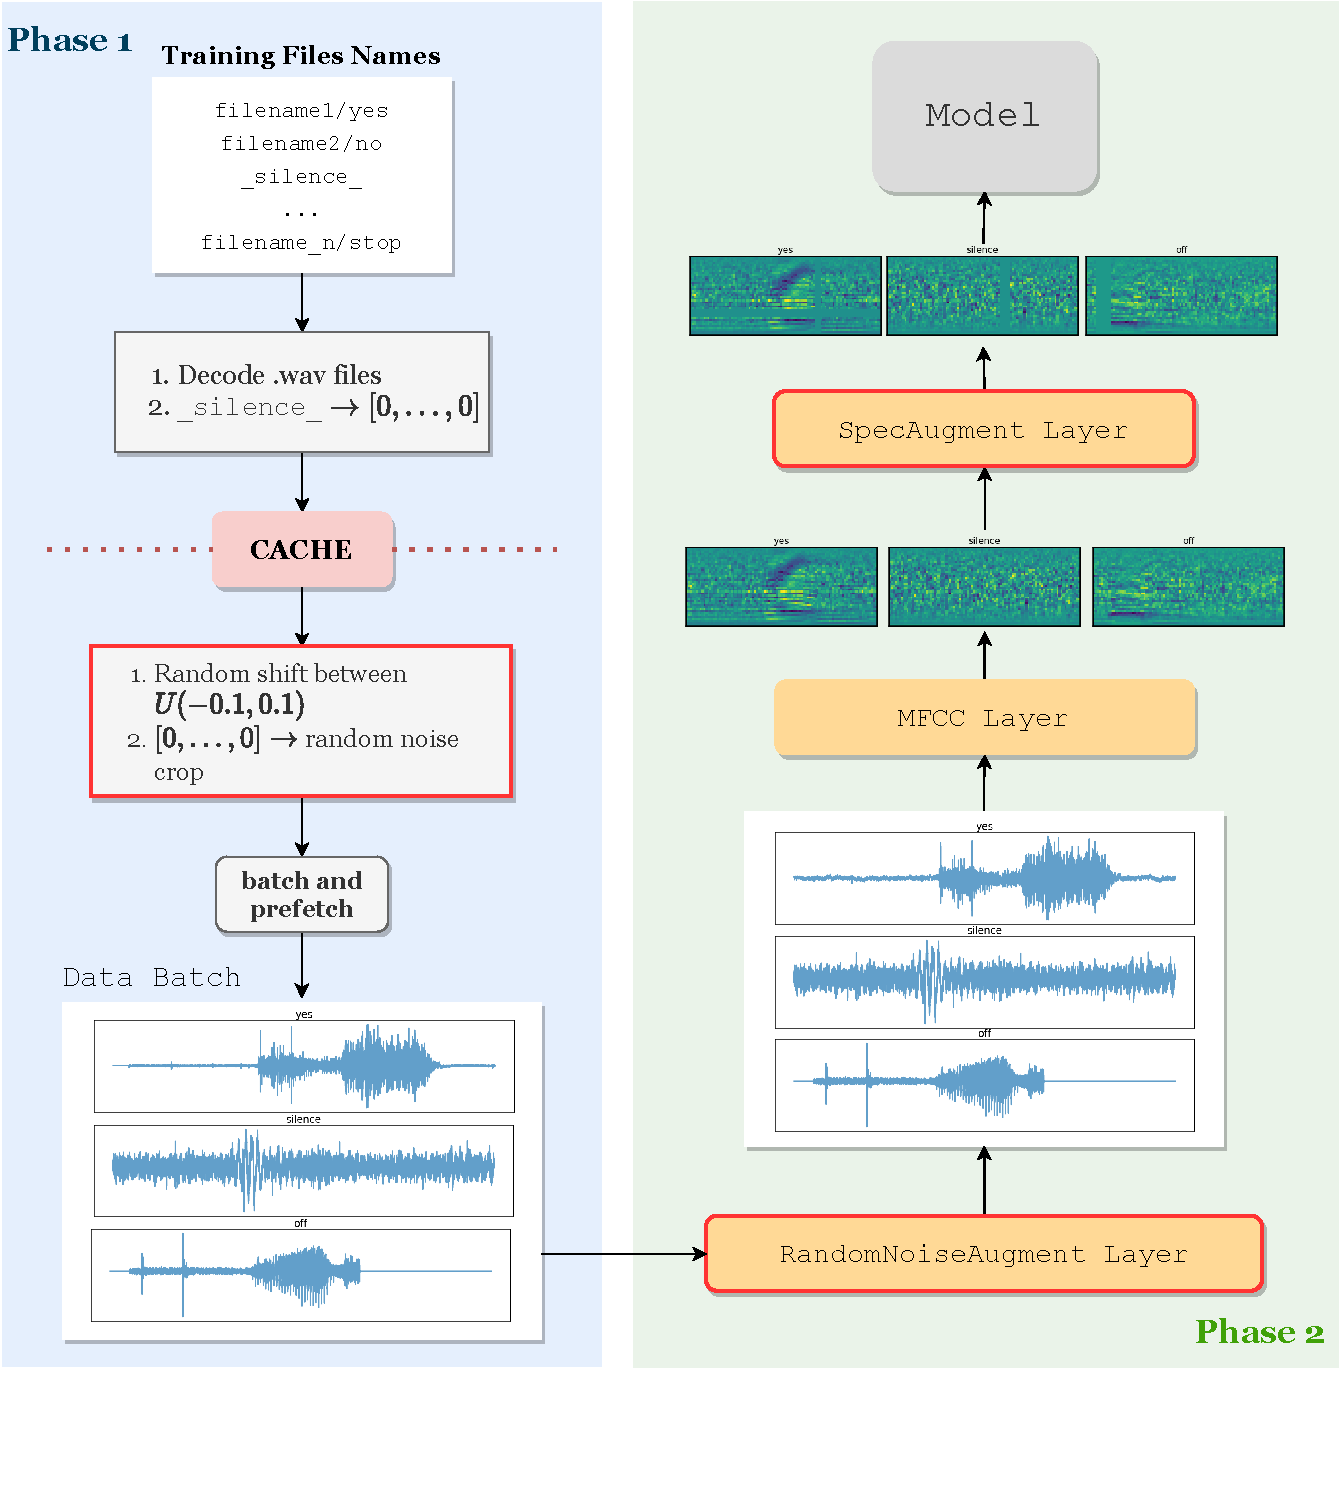
\includegraphics[width=0.99\linewidth]{imgs/input_pipeline_v3.pdf}
	%TODO: image is still wip
	\caption{Detailed description of the input pipeline for the training data. In the cache block, the data that was produced until that moment is saved to file. Each step which is performed before the caching operation happens only one time, during the first iteration of the dataset; on all the successive iterations, the data is read from the cached file. Boxes with the red outline denote data augmentation steps}
	\label{fig:inputpipeline}
\end{figure}





\subsection{Learning Framework}
\label{sec:learning_framework}

We now describe each proposed architecture, mainly using summary tables. Note that each RNN layer is bidirectional, each CNN layer uses stride $=(1,1)$, padding = \verb|same|, and uses batch normalization before passing through the activation function. Also, the first layers of each model are the preprocessing layers discussed in the previous section; here we don't report them as they are not part of the actual model architecture. In the tables we report with $m$ the number of output classes, which differ depending on the type of task. Finally, we denote with \say{Attention} the attention layer used by Att-RNN, while with \say{QAttention} we mean the attention layer introduced for SQAtt-RNN. For all multi-head attention layers, the projection dimension is set to $64$.

\subsubsection{\textbf{SimpleAtt}}
We propose this model as a baseline light weight model to see how its performances compare to more complex architectures. It's architecture is shown in Table \ref{tab:simpleatt_architecture}.

\begin{table}[h!]
	\caption{Simple Attention RNN architecture}
	\label{tab:simpleatt_architecture}
	\scalebox{0.9}{
	\begin{tabular}{|c|c|c|c|c|c|c|}
		\hline
		layer type & $n$RNN & $n$MLP & $n$F & Fw & Fh & Act.    \\ \hline
		RNN (GRU)  & $64$   &      &    &    &    & tanh    \\ \hline
		Attention  &      &      &    &    &    &         \\ \hline
		Dense      &      & $128$  &    &    &    & ReLu    \\ \hline
		Dense      &      & $64$   &    &    &    & ReLu    \\ \hline
		Dense      &      & $m$  &    &    &    & Softmax \\ \hline
	\end{tabular}}
\end{table}
\subsubsection{\textbf{Att-RNN}}
The baseline model, from \cite{attention2018andreade}. Architecture is shown in Table \ref{tab:attrnn_architecture}.

\begin{table}[h!]
	\caption{Att-RNN architecture}
	\label{tab:attrnn_architecture}
	\scalebox{0.9}{
	\begin{tabular}{|c|c|c|c|c|c|c|}
	\hline
	layer type & $n$RNN & $n$MLP & $n$F & Fw & Fh & Act.    \\ \hline
	Conv       &      &      & $10$ & $5$  & $1$  & ReLu    \\ \hline
	Conv       &      &      & $1$  & $5$  & $1$  & ReLu    \\ \hline
	RNN (LSTM) & $128$  &      &    &    &    & tanh    \\ \hline
	RNN(LSTM)  & $128$  &      &    &    &    & tanh    \\ \hline
	Attention  &      &      &    &    &    &         \\ \hline
	Dense      &      & $64$   &    &    &    & ReLu    \\ \hline
	Dense      &      & $m$  &    &    &    & Softmax \\ \hline
\end{tabular}}
\end{table}

\subsubsection{\textbf{SQAtt-RNN}}
Simple variation of Att-RNN, where the attention layer is modified in order to return a new sequence. The idea is that the new returned sequence will constitute a richer representation of the input sequence. Architecture is shown in Table \ref{tab:sqattrnn_architecture}.

\begin{table}[h!]
		\caption{SQAtt-RNN architecture}
	\label{tab:sqattrnn_architecture}
	\scalebox{0.9}{
	\begin{tabular}{|c|c|c|c|c|c|c|}
		\hline
		layer type & nRNN & nMLP & nF & Fw & Fh & Act.    \\ \hline
		Conv       &      &      & 10 & 5  & 1  & ReLu    \\ \hline
		Conv       &      &      & 1  & 5  & 1  & ReLu    \\ \hline
		RNN (GRU)  & 128  &      &    &    &    & tanh    \\ \hline
		RNN (GRU)  & 128  &      &    &    &    & tanh    \\ \hline
		QAttention &      &      &    &    &    &         \\ \hline
		RNN (GRU)  & 64   &      &    &    &    & tanh    \\ \hline
		Dense      &      & 64   &    &    &    & ReLu    \\ \hline
		Dense      &      & $m$  &    &    &    & Softmax \\ \hline
	\end{tabular}}
\end{table}

\subsubsection{\textbf{SQ-noCNN}}
Simple variation of SQAtt-RNN, where we completely omit the CNN block. This is done to investigate the impact of the initial feature extraction phase performed by the Convolutional layers. In this way, the input to the RNN block is the raw feature matrix.

\subsubsection{\textbf{MHAtt-RNN}}
Variation of Att-RNN, proposed in \cite{streamingkws2020Rybakov}. We train different versions of this architecture, varying the number of heads. Architecture is shown in Table \ref{tab:mhattrnn_architecture}.

\begin{table}[h!]
	\centering
	\caption{MHAtt-RNN$h$ architecture, where $h$ is the number of heads for the MH Attention layer.}
	\label{tab:mhattrnn_architecture}
	\scalebox{0.9}{
	\begin{tabular}{|c|c|c|c|c|c|c|}
		\hline
		layer type   & $n$RNN & $n$MLP & $n$F & Fw  & Fh  & Act.     \\ \hline
		Conv         &        &        & $10$ & $5$ & $1$ & ReLu             \\ \hline
		Conv         &        &        & $1$  & $5$ & $1$ & ReLu              \\ \hline
		RNN (GRU)    & $128$  &        &      &     &     & tanh              \\ \hline
		RNN (GRU)    & $128$  &        &      &     &     & tanh              \\ \hline
		MHAttention &        &        &      &     &     &               \\ \hline

		Dense        &        & $64$   &      &     &     & ReLu             \\ \hline
		Dense        &        & $m$    &      &     &     & Softmax          \\ \hline
	\end{tabular}}
\end{table}

\subsubsection{\textbf{SQMHAtt-RNN}}
Variation of MHAtt-RNN, where we use the whole sequence as query vectors in the same way it is done in SQAtt-RNN.

\subsubsection{\textbf{Res-Att}}
Variation of Att-RNN where we use a deeper CNN block, constituted of residual layers.  We train different versions of this architecture, varying the number of resdual blocks used. The residual block is shown in Figure \ref{fig:resblock}. We report the whole architecture in Table \ref{tab:resatt_architecture}. 

\begin{figure}
	\centering
	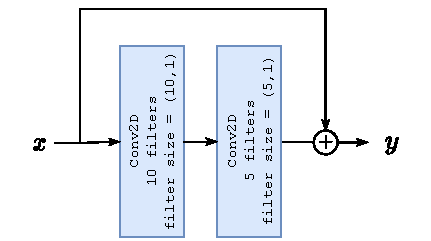
\includegraphics[width=0.9\linewidth]{imgs/residual_block.pdf}

	\caption{Architecture for the residual block used in the Res-Att model.}
		\label{fig:resblock}
\end{figure}

\begin{table}[h!]
	\centering
	\caption{Res-Att$k$ architecture, where $k$ is the number of residual blocks.}
	\label{tab:resatt_architecture}
	\scalebox{0.9}{
	\begin{tabular}{|c|c|c|c|c|c|c|}
		\hline
		layer type            & $n$RNN & $n$MLP & $n$F & Fw  & Fh  & Act.    \\ \hline
		Conv                  &        &        & $5$  & $5$ & $1$ & ReLu    \\ \hline
		ResBlock ($\times k$) &        &        &      &     &     &         \\ \hline
		Conv                  &        &        & $1$  & $5$ & $1$ & ReLu    \\ \hline
		AvgPool $(2,1)$       &        &        &      &     &     &         \\ \hline
		RNN (GRU)             & $128$  &        &      &     &     & tanh    \\ \hline
		RNN (GRU)             & $128$  &        &      &     &     & tanh    \\ \hline
		Attention             &        &        &      &     &     &         \\ \hline
		Dense                 &        & $64$   &      &     &     & ReLu    \\ \hline
		Dense                 &        & $m$    &      &     &     & Softmax \\ \hline
	\end{tabular}}
\end{table}


Each model was trained for 30 epochs, using the Adam optimizer with a starting learning rate of $0.001$. To learn as much as possible, in the case where after 2 epochs the validation loss didn't improve, the learning rate was reduced of a factor of $0.1$.

%Here you finally describe the learning strategy / algorithm that you conceived and used to solve the problem at stake. A good diagram to exemplify how learning is carried out is often very useful. In this section, you should describe the learning model, its parameters, any optimization over a given parameter set, etc. You can organize this section into \mbox{sub-sections}. You are free to choose the most appropriate structure.
%
%\begin{remark}
%Note that the diagram that you put here differs from that of Section~\ref{sec:processing_architecture} as here you show the details of how your learning framework, or the core of it, is built. In Section~\ref{sec:processing_architecture} you instead provide a high-level description of the involved processing blocks, i.e., you describe the {\it processing flow} and the rationale behind it.
%\end{remark}
%
%
%


% !TEX root = template.tex

\section{Results}
\label{sec:results}

In Table \ref{table:results} we report the different accuracies...
%
%In this section, you should provide the numerical results. You are free to decide the structure of this section. As a general ``rule of thumb'', use plots to describe your results, showing, e.g., precision, recall and \mbox{F-measure} as a function of the system (learning) parameters. You can also show the precision matrix. 
%
%\begin{remark}
%Present the material in a progressive and logical manner, starting with simple things and adding details and explaining more complex findings as you go. Also, do not try to explain/show multiple concepts within the same sentence. Try to \textbf{address one concept at a time}, explain it properly, and only then move on to the next one.
%\end{remark}
%
%\begin{remark}
%The best results are obtained by generating the graphs using a vector type file, commonly, either \texttt{encapsulated postscript (eps)} or \texttt{pdf} formats. To plot your figures, use the Latex \texttt{\textbackslash includegraphics} command. Lately, I tend to use pdf more.
%\end{remark}
%
%\begin{remark}
%If your model has hyper-parameters, show selected results for several values of these. Usually, tables are a good approach to concisely visualize the performance as hyper-parameters change. It is also good to show the results for different flavors of the learning architecture, i.e., how architectural choices affect the overall performance. An example is the use of CNN only or CNN+RNN, or using inception for CNNs, dropout for better generalization or attention models. So you may obtain different models that solve the same problem, e.g., CNN, CNN+RNN, CNN+inception, etc.
%\end{remark}
\begin{table}
	\caption{Table with results}
\begin{tabular}{lccc}
	
	\hline 
	Model & Param. & Mult. & Acc. \\
	\hline \hline
	
	res8-narrow[7] & $20 \mathrm{~K}$ & $5.65 \mathrm{M}$ & $90.1 \%$ \\
	res15-narrow[7] & $43 \mathrm{~K}$ & $160 \mathrm{M}$ & $94.0 \%$ \\
	res8[7] & $111 \mathrm{~K}$ & $30 \mathrm{M}$ & $94.1 \%$ \\
	res15[7] & $239 \mathrm{~K}$ & $894 \mathrm{M}$ & $95.8 \%$ \\
	\hline 
	DS-CNN-S[5] & $24 \mathrm{~K}$ & $5.4 \mathrm{M}$ & $94.4 \%$ \\
	DS-CNN-M[5] & $140 \mathrm{~K}$ & $19.8 \mathrm{M}$ & $94.9 \%$ \\
	DS-CNN-L[5] & $420 \mathrm{~K}$ & $56.9 \mathrm{M}$ & $95.4 \%$ \\
	\hline TC-ResNet8[8] & $66 \mathrm{~K}$ & $1.12 \mathrm{M}$ & $96.1 \%$ \\
	TC-ResNet8-1.5[8] & $145 \mathrm{~K}$ & $2.20 \mathrm{M}$ & $96.2 \%$ \\
	TC-ResNet14[8] & $137 \mathrm{~K}$ & $2.02 \mathrm{M}$ & $96.2 \%$ \\
	TC-ResNet14-1.5[8] & $305 \mathrm{~K}$ & $4.13 \mathrm{M}$ & $\mathbf{9 6 . 6 \%}$ \\
	\hline TENet6-narrow & $\mathbf{1 7 K}$ & $\mathbf{5 5 3 K}$ & $96.0 \%$ \\
	TENet12-narrow & $31 \mathrm{~K}$ & $895 \mathrm{~K}$ & $96.3 \%$ \\
	TENet6 & $54 \mathrm{~K}$ & $1.68 \mathrm{M}$ & $96.4 \%$ \\
	TENet12 & $100 \mathrm{~K}$ & $2.90 \mathrm{M}$ & $\mathbf{9 6 . 6 \%}$ \\
	\hline
	
	\label{table:results}
\end{tabular}
\end{table}

% !TEX root = template.tex

\section{Concluding Remarks}

In this work, we explored different variants of attention based models for keyword spotting. In particular, we found that models based on multi head attention provide slightly higher accuracy with respect to the baseline Att-RNN  model, even if this came with the cost of a higher parameter count. Deeper convolutional blocks didn't prove to be beneficial, even if this could be due to a too simplistic design for the residual layers. Similarly to many works in the literature, we used the top-1 accuracy as the only metric, but this is not a complete way to evaluate a KWS model. For example, authors in \cite{dnns2014chen}\cite{convnns2015sainath}\cite{streamingkws2020Rybakov} make audio streaming tests to evaluate the false reject and false alarm rate, as well as system latency, to have additional tools for evaluation. Also, for this project the models were trained just one time due to the limited computational capabilites; this fact makes the reported results not too statistically relevant. To perform a more rigorous statistical analysis, one should train the models more times and use an avarage of the test set accuracies among the runs, computing confidence intervals for the final accuracy. Furthermore, additional experiments regarding attention mechanisms could be done starting from the Keyword Transformer architecture; even if the KWT has an extremely heavy memory footprint, it could be worth experimenting lighter variations of it.

In conclusion, this was a very instructive project to work on: I had the opportunity to study a lot of modern machine learning literature and to understand more complex architectures based on the attention mechanism. I also think that this report \LaTeX template was extremely useful and well done, and it will surely be a very useful tool for the future. Besides the part involving the study of the literature, the most difficult part of this work, in my experience, was to build a working input pipeline, both for technical reasons (due to the limitations of my hardware) and for the difficulty to find information online. While it is true that the Labs were extremely useful and essential, especially on the part regarding the \verb|tf.data.Dataset| API, while working on the project I often came across errors which were really hard to debug mostly because of my unawareness of how Tensorflow really works under the hood (see for example the difference between Graph execution and Eager execution). Besides this aspect, I think that the course gave me strong knowledge foundations in order to complete the project.

\label{sec:conclusions}
%
%\red{This section should take max half a page, I personally find it difficult to come up with really useful observations, I mean ones that bring a new contribution with respect to what you have already expounded in the ``Results'' section. In case you have some serious stuff to write, you may also extend the section to 3/4 of a page :-).}\\
%
%In many papers, here you find a summary of what done. It is basically an abstract where instead of using the present tense you use the past participle, as you refer to something that you have already developed in the previous sections. While I did it myself in the past, I now find it rather useless.\\ 
%
%\MR{\textbf{What I would like to see here is:} 
%\begin{enumerate}
%\item a very short summary of what done, 
%\item some (possibly) intelligent observations on the relevance and {\it applicability} of your algorithms / findings, 
%\item what is still missing, and can be added in the future to extend your work.\\
%\end{enumerate}
%The idea is that this section should be {\it useful} and not just a repetition of the abstract (just \mbox{re-phrased} and written using a different tense...).}\\
%
%\red{\textbf{Moreover:} being a project report, I would also like to see a specific paragraph stating 
%\begin{enumerate}
%\item[4)] what you have learned, and 
%\item[5)] any difficulties you may have encountered.
%\end{enumerate}}


\bibliography{biblio}
\bibliographystyle{ieeetr}

\end{document}


